\documentclass[11pt]{article}

\usepackage{graphicx}


\title{PROGETTO BASI DI DATI 22/23 \\ Bisogna inserire cose più fighe tipo \\ UNIVERSITA' FEDERICO SECONDO con l'immagine \\ aggiunger un sommario \\ etc }

\author{Adolfo Torcicollo \\ Francesca Pugliese}
\date{}  												%da aggiungere
\begin{document}
	
	\part{Descrizione del progetto}
	\section{Analisi del problema}
	
	Si progetterà e svilupperà una base di dati di tipo relazionale\\ per la gestione di progetti di un’azienda. \\
	
	\section{Approccio al problema}
	
	A fronte di un’analisi, è stato scelto di gestire la piattaforma\\ che fa uso della base di dati in questione \\
	in modo totalmente indipendente rispetto agli strumenti utilizzati per la gestione di altre funzionalità di un app musicale.\\
	Inoltre, non si tratta di un programma pubblico e aperto;\\ pertanto, nella progettazione della base di dati è stato scelto di omettere 
	informazioni non indispensabili.\\
	
	\section{Informazioni da analizzare}
	
	La base di dati deve garantire alla piattaforma che ne fa uso i seguenti servizi:
	\footnote{INSERIRE ROBA QUI, dove leggi il numero 1}
	\\
	Il database è stato pensato in stretta relazione con l’applicativo; pertanto, in fase di \\ 
	progettazione si è deciso di ripartire il carico di operazioni e vincoli tra entrambe le parti.\\
	
	\clearpage
	
	\part{Progettazione concettuale}
	\section{Class Diagram}
	In questo capitolo verrà riportato il class diagram realizzato in fase di progettazione \\

	\begin{figure}
		\centering
		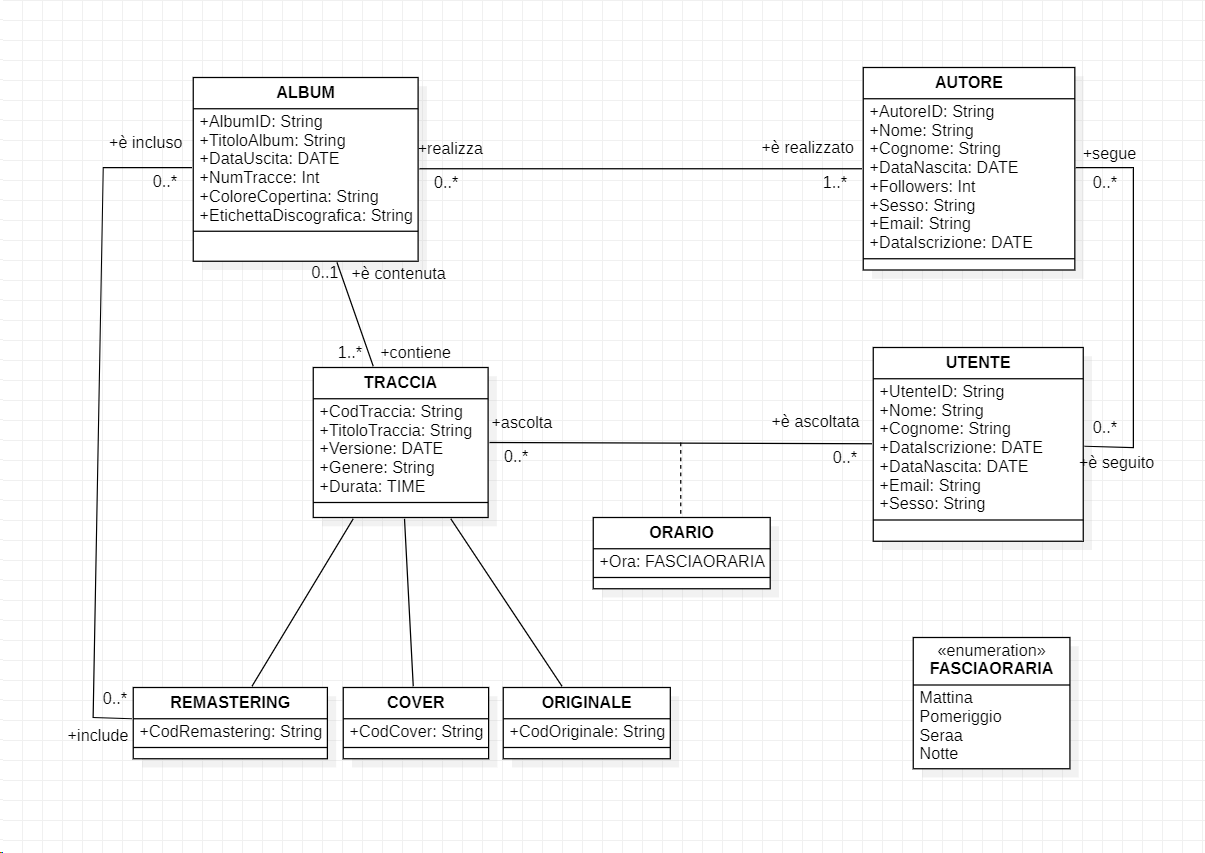
\includegraphics[width=1\linewidth]{SpotifyPezzotto.png}
		\caption{}
		\label{spotifypezzotto}
	\end{figure}
	
	\clearpage
\end{document}